
\section{Introduction}

% Make the introduction more elaborate
% Introduce terms such as lubrication film, film thickness and lubrication regime.
% Introduce active, passive, invasive, non-invasive methods
% Introduce online, atline, inline, offline sensing methods
% Introduce signal processing in the lubrication condition monitoring framework

Lubrication of ball bearings is essential for reducing friction, wear and overheating \cite{wakiru_review_2019} \cite{isalm_oil_2021}. Inadequate or excessive lubrication can lead to increased wear, higher operating temperatures, and ultimately premature failure of the bearing. Improper lubrication is estimated to be the cause of between 30\% to 80\% of ball bearing failures but the lubrication condition monitoring (LCM) has not received the same attention as the well documented vibration analysis used for both fault detection and remaining useful life (RUL) estimation \cite{jakobsen_detecting_2023} \cite{dai_situ_2024} \cite{xu_vibration-based_2024} \cite{nassef_impact_2022}.

LCM of ball bearings covers the problems of estimating the film thickness, viscosity, degradation, and contamination from wear debris and environmental factors of the lubricant as well as rolling friction resulting from the conditions in the bearing. This in general is related to the ability of the lubricant to reduction friction and wear of the ball bearing.

This review aims to provide an overview of the current state of research in the field of online LCM for ball bearings. The review focuses on theoretical models of lubrication in ball bearings, sensing methods, signal processing techniques, and their applications in detecting lubrication degradation and film thickness changes.

% Finally, the review indentifies gaps in the existing literature and suggests potential areas for future research. \todo{Make sure to follow up on the identified gaps and areas for future research.}

\subsection{Monitoring Flow}
Online LCM relies upon information gathering during operation of ball bearings and consists of three or four distinct processes:
\begin{enumerate}
    \item Sensing methods: observation and data collection from a ball bearing in operation through sensors.
    \item Feature extraction: manipulation and analysis of the collected data through signal processing and machine learning.
    \item Lubrication condition assessment: classification or regression of the processed data in order to infer lubrication conditions in the bearing.
    \item Maintenance decision: a concrete relubrication strategy based upon the lubrication condition assessment. This includes when and how much to lubricate in order to maintain or restablish preferred lubrication conditions.
\end{enumerate}
The steps in LCM related to the maintenance of a ball bearing are visualized in Figure \ref{fig:lcm_flow}. LCM is concerned mainly with inference on the lubrication conditions which stricly speaking does not include the maintenance decisions. The maintenance decision can, however, be included for a complete pipeline.

\begin{figure}[!h]
\centering
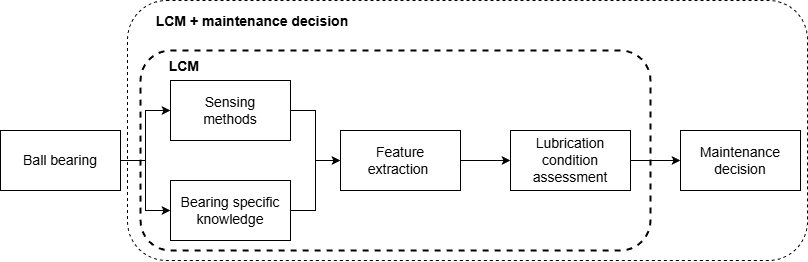
\includegraphics[width=0.9\textwidth]{figures/lcm_overview.png}
\caption{Steps in the process of maintenance of a running ball bearing with online LCM.}
\label{fig:lcm_flow}
\end{figure}

\subsection{Existing Reviews}
A number of reviews on lubrication condition monitoring in ball bearings have been conducted:
\begin{itemize}
    \item \cite{wakiru_review_2019} reviews the use of lubrication condition monitoring for maintenance decision support. The authors mainly cover direct analysis of used lubricant resulting in variables characterizing the physical and chemical state of the lubricant as well as the mathematical models used for maintenance decision support. The sensing methods covered are invasive.
    \item \cite{shang_comprehensive_2024} reviews the estimation of lubrication film thickness in bearings through the use of optical, electrical and ultrasonic sensing methods along with the physics models used for interpretation of the signals. It is concluded that the optical method is highly sensitive to film thickness but requires either unobstructed observation paths or alterations of the bearing structures. The electrical method requires highly sensitive sensors and the ultrasonic method is highly dependent on the bearing material and operating environment. All methods are active or invasive.
    \item \cite{wang_advanced_2024} reviews bearing condition monitoring methods which includes detection of wear debris in the lubricant and lubricant film thickness. The lubricant analysis methods include offline lubricant laboratory analysis, ion-selective sensors mounted in the lubricant and magnetic methods relying on ferromagnetic or inductive sensors to detect debris content. All sensing methods are active or invasive.
    % It is furthermore noted that ultrasonic sensors can be used for film thickness estimation, electrostatic sensors can be used for passive, non-invasive debris detection and thermocouples or infrared sensors can measure increased friction as a result of inadequate lubrication through heat generation. The signal processing and models used for lubrication condition monitoring encompass time domain statistics as well as machine learning for classification and dimensionality reduction.
    \item \cite{hansen_comparison_2022} reviews calibration methods for ultrasonic reflectometry. The methods are active and rely on ultrasonic waves induced into the bearing.
    \item \cite{cen_ehl_2021} reviews the electrical capacitance methods which treats the bearing as a capacitor with the rolling elements and raceways acting as plates. The change in capacitance during operation can then be attributed to a change in the lubricant film between the plates.
    \item \cite{becker-dombrowsky_electrical_2024} similarly reviews electrical impedance based methods which seek to estimate the film thickness through changes in the impedance of the ball bearing system.
    \item \cite{dai_situ_2024} also reviews film thickness estimation based upon electrical capacitance models which rely on active sensors.
    \item \cite{zhu_lubricating_2017} reviews online sensors for measuring lubricant properties but does not directly concern bearings. The authors mention sensors using magnetic induction, electrical capacitance, ultrasnoic emission and optical properties. All of the sensors are active and/or invasive.
    \item \cite{sun_online_2021} reviews methods for monitoring debris content of lubricants which is related to wear of rotating machinery. The authors classify sensing methods into magnetic, electrical, optical and acoustic which are all active methods with the exeption of a ferromagnetic method.
    \item \cite{dou_review_2022} reviews the ultrasonic reflection technology for estimating film thickness in lubricants. The review does not specifically concern bearings and the sensing mehods are active.
    \item \cite{zhu_survey_2013} reviews lubrication oil monitoring methods and classifies them into electrical (magnetic), physical, chemical and opticel methods. The methods are all either active or invasive. Ball bearings are not specifically mentioned.
\end{itemize}

\subsection{Existing Industrial Applications}
Ultrasound is currently being used in the industry for passive, non-invasive, online LCM, e.g. through the Ultraprobe from UE Systems. This methods relies on a simple threshold model which establishes a reference level of ultrasound when the bearing is adequately lubricated and instructs to relubricate when the ultrasound energy level rises above a certain threshold set relative to the reference.